\documentclass{report}
\usepackage{fullpage}
\usepackage{graphicx}
\usepackage{subfigure}
\usepackage[font=small,skip=1pt]{caption}
\usepackage{booktabs}
\usepackage{amsmath}


\renewcommand{\baselinestretch}{2}




\author{Abdullah-Al-Zubaer Imran\\Curtis Crawford}
\title{University of California, Los Angeles \\
		{\large EE219: \textbf{Classification} \\ Project Report} }  
\date{}





\begin{document}
\maketitle

\section*{Introduction}
Clustering alogrithms find groups of data points that have similar representations in a proper space, in unsupervised way. Clustering differs from classification in that without having any prior labelling of the data points. K-means clustering is a clustering technique that interatively groups data points into regions characterized by a set of cluster centroids. Data representation is very crucial for any clustering algorithm like K-means. In this project, we have figured out proper representations of the data points so that we can get efficient and reasonable results from the clustering. Then we performed K-means clutering on the dataset and evaluated performance using different performance measures. Moreover, different preprocess techniques were performed for possible increase in performance of the clusering. 

\section*{Dataset}
For this project, we have used "20 Newsgroups" dataset which is a collection of approximately 20,000 documents, partitioned evenly across 20 different newsgroups, each corresponding to a different topic. And each topic is viewed as a class. Since we performed clustering on this dataset, we pretended that the class labels are not available in the dataset. 



\section*{Wroking Procedures \& Results}

\subsection*{Data Representation}
In order to find a good representation of the data, the documents were transformed into TF\--IDF vectors using min\_df = 3.
The Tf\--IDF matrix dimension: (7882, 27768)   \\

\subsection*{Clustering}
Then we applied K-means clustering with k = 2 to determine the groups or classes the data points belong to, without providing any prior label. For evaluation purpose, we re-labeled data with either 0 for comp-tech or 1 for rec. And compared the clustering results with the known labels. \\ 


\subsubsection*{Performance Measures}
In addition to this, we examined several measures to make a concrete comparison of the clustering results. Results from different measures are reported in the following table: 

\begin{center}
	\textbf{Performance metrics' scores for clustering}	
	\begin{tabular}{*{2}{c}}
		\toprule
		\textbf{Measure} & \textbf{Score}  \\
		\midrule
		Homogeneity: & 0.791324640919  \\
		\midrule
		Completeness: & 0.79150685559   \\
		\midrule
		V-measure: & 0.791415737766   \\
		\midrule
		Rand: & 0.872390054996   \\
		\midrule
		Mutual info: & 0.79130553663  \\
		\bottomrule
	\end{tabular}
	\qquad
	$Contigency = \left[\begin{array}{*{2}{c}}
    				151 & 3752 \\
     				3870 & 109
					\end{array}\right]
					$
\end{center}    

\\  \vspace{20pt}



\subsection*{Data Preprocessing}
As we observe from the clustering result, TF\--IDF vector did not yield a good result for K-means clustering. Therefore, we tried with better representations of the data. We performed two dimensionality reduction techniques as the preprocess for K-means clustering. \\ \vspace{10pt}


\subsubsection{Dimensionality Reduction}
We have used Latent Semantic Indexing (LSI) and Non-negative Matrix Factorization (NMF) for dimensionality reduction. 
We determined the effective dimension of the data through inspection of the top singular values of the TF\--IDF matrix and noticed how many of them are significant in reconstructing the matrix with the truncated SVD representation. We checked what ratio of the variance of the original data is retained after dimensionality reduction. Figure \ref{fig:variance_r} shows the plot of the percent of variance the top r principle components can retain vs. r, for r = 1 to 1000.

\begin{figure}
  \centering
  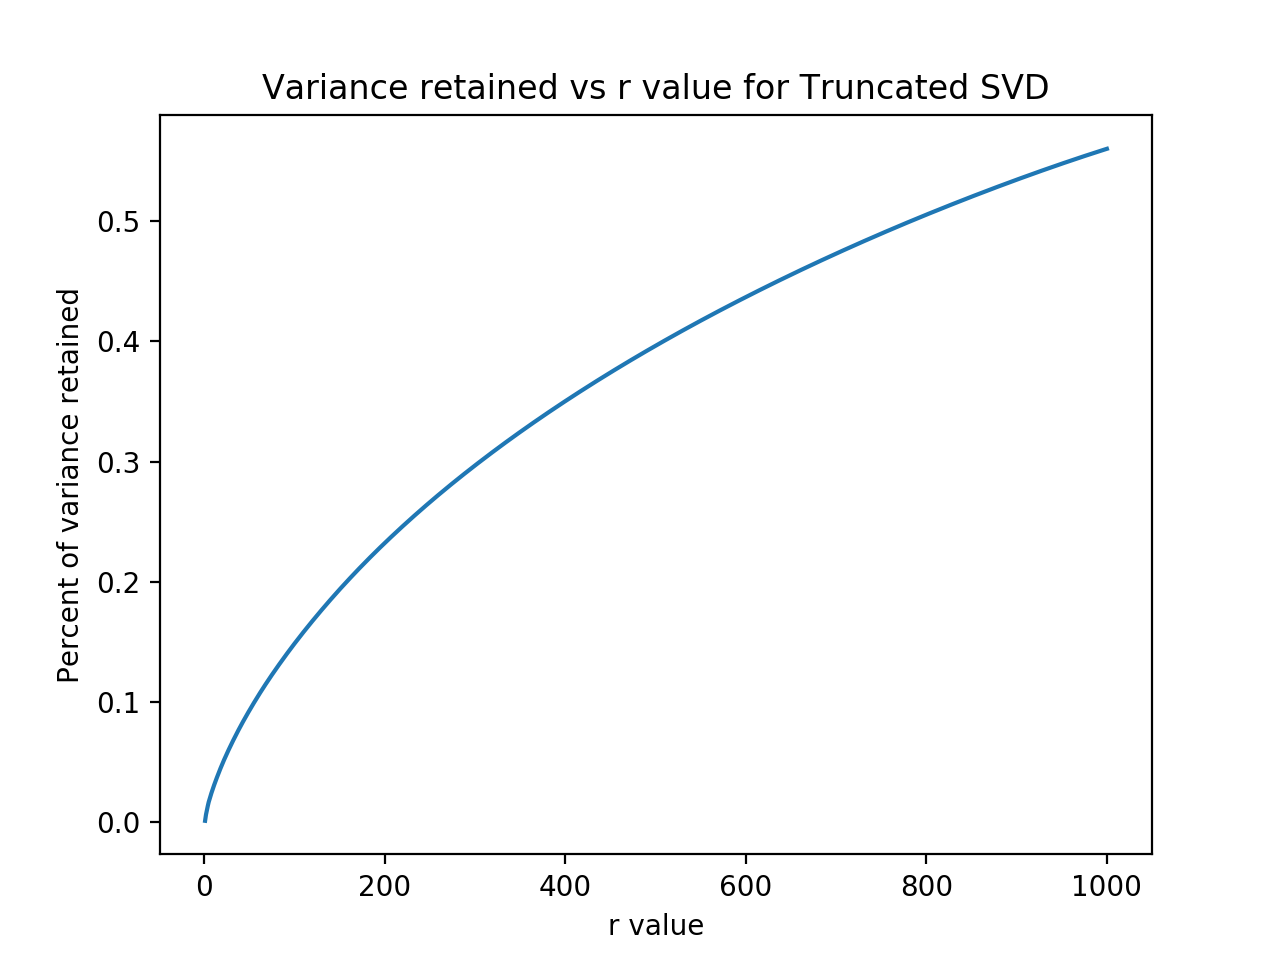
\includegraphics[width=\linewidth]{p3_variance_r.png}
  \vspace*{-20mm}
  \caption{Plot of the Percent of variance retained in PCA vs. r.}
  \label{fig:variance_r}
\end{figure}

For dimensionality reduction, we used LSI and NMF methods. We swept over the parameters for each method (LSI and NMF) to determine the one yielding better results in terms of clustering metrics. All five performance metrics for clustering with different r-values are reported below. \\


\underline{\textbf{NMF with r = 1}} 

\begin{center}
	\textbf{Performance metrics's scores for the clustering} \\ \vspace{10pt}
	\begin{tabular}{*{2}{c}}
		\toprule
		\textbf{Measure} & \textbf{Score} \\
		\midrule	
		Homogeneity: & 0.000311084586659 \\
		\midrule
		Completeness: & 0.00031474279897 \\
		\midrule
		V-measure: & 0.000312903000955 \\
		\midrule
		RAND: & 0.000349910576703 \\
		\midrule
		Mutual Info: & 0.000219562406476 \\
		\bottomrule
	\end{tabular}
	\qquad
	$Contigency = \left[ \begin{array}{*{2}{c}}
			    1744 & 2159\\
			    1696 & 2283				
				\end{array}\right]
			$
\end{center}

\\  \\ \vspace{20pt}


\underline{\textbf{SVD with r = 1}} 

\begin{center}
	\textbf{Performance metrics' scores} \\  \vspace{10pt}
	\begin{tabular}{*{2}{c}}		
		\toprule
		\textbf{Measure} & \textbf{Score} \\
		\midrule
		Homogeneity: & 0.000310977615107 \\
		\mdirule 
		Completeness: & 0.000314664424341 \\
		\midrule
		V-measure: & 0.000312810156833  \\
		\midrule
		RAND score: & 0.000349914958924  \\
		\midrule
		Mutual Info:  & 0.000219455422027 \\
		\bottomrule
	\end{tabular}
	\qquad
	$Contingency = \left[\begin{array}{*{2}{c}}
		 2160	& 1743 \\
 		 2284 	& 1695 \\ 
			\end{array}\right]
		$
\end{center}

\newpage


\\
\underline{\textbf{NMF with r = 2}} 
\begin{center}
	\textbf{Peformance metrics's scores} \\  \vspace{10pt}
	\begin{tabular}{*{2}{c}}
		\toprule
		\textbf{Measure} & \textbf{Score} \\
		\midrule
		Homogeneity: & 0.592844515412 \\
		\midrule
		Completeness: & 0.608067163036 \\
		\midrule
		V-measure: 	& 0.600359358773 \\
		\midrule
		RAND score: & 0.648591716894 \\
		\midrule
		Mutual Info:	& 0.592807239875 \\
		\bottomrule
	\end{tabular}
	\qquad	
	$Contingency = \left[\begin{array}{*{2}{c}}
 		731	& 3172 \\
 		3943 & 36 
				\end{array}\right]
	$
\end{center}
\\  \\ \vspace{20pt}



\underline{\textbf{SVD with r = 2}} 

\begin{center}
	\textbf{Peformance metrics's scores} \\  \vspace{10pt}
	\begin{tabular}{*{2}{c}}
		\toprule
		\textbf{Measure} & \textbf{Score} \\
		\midrule
		Homogeneity: & 0.608223241581 \\
		\midrule
		Completeness: & 0.608333021975 \\
		\midrule
		V-measure: & 0.608278126825 \\
		\midrule
		RAND: & 0.713926529273 \\
		\midrule
		Mutual Info: & 0.608187374307 \\
		\bottomrule
	\end{tabular}
	\qquad
	$Contingency = \left[\begin{array}{*{2}{c}}
		250 & 3653 \\
		3618 & 361 
			\end{array}\right]
		$
\end{center}
\newpage


\underline{\textbf{NMF with r = 3}} 

\begin{center}
	\textbf{Performance metrics' scores} \\ \vspace{10pt}	
	\begin{tabular}{*{2}{c}}
		\toprule
		\textbf{Measure} & \textbf{Score} \\
		\midrule
		Homogeneity: & 0.237561424862 \\
		\midrule
		Completeness: 		& 0.317099662339 \\
		\midrule
		V-measure:			& 0.271627663619 \\
		\midrule
		RAND score: 		& 0.16950318518 \\
		\midrule
		Mutual Info: 		& 0.237491614778 \\
		\bottomrule
	\end{tabular}
	\qquad
	$Contingency = \left[\begin{array}{*{2}{c}}
		13 & 3890 \\
		1674 & 2305 \\
			\end{array}\right]
		$
\end{center}
\\  \vspace{20pt}


\underline{\textbf{SVD with r = 3}} 

\begin{center}
	\textbf{Performance metrics' scores} \\ \vspace{10pt}	
	\begin{tabular}{*{2}{c}}	
		\toprule
		\textbf{Measure} & \textbf{Score} \\ 
		\midrule
		Homogeneity: & 0.0353596802034 \\
		\midrule 
		Completeness: & 0.165160546781 \\
		\midrule
		V-measure: 	& 0.0582487283625 \\
		\midrule
		RAND score: & 0.00593193880668 \\
		\midrule
		Mutual Info: & 0.0352712181601 \\
		\bottomrule
	\end{tabular}
	\qquad
	$Contingency = \left[ \begin{array}{*{2}{c}}
		3635 & 268 \\
		3979 & 0   
        \end{array}\right]
		$
\end{center}
\newpage

\underline{\textbf{NMF with r = 5}} 
\begin{center}
	\textbf{Performance metrics scores} \\ \vspace{10pt}	
	\begin{tabular}{*{2}{c}}
		\toprule
		\textbf{Measure} & \textbf{Score} \\
		\midrule		
		Homogeneity: & 0.125884883543 \\
		\midrule
		Completeness: & 0.127229904183 \\
		\midrule
		V-measure: & 0.126553820227 \\
		\midrule
		RAND score: & 0.165339719484 \\
		\midrule
		Mutual Info: & 0.125804857758 \\
		\bottomrule
	\end{tabular}
	\qquad
	$Contingency = \left[ \begin{array}{*{2}{c}}
		2992  & 911 \\
		1427  & 2552 
		\end{array}\right]
		$
\end{center}
\\ \vspace{20pt}

\underline{\textbf{SVD with r = 5}} 

\begin{center}
	\textbf{Performance metrics' scores} \\ \vspace{10pt}	
	\begin{tabular}{*{2}{c}}
		\toprule
		\textbf{Measure} & \textbf{Score} \\	
		\midrule
		Homogeneity: & 0.138545661957 \\
		\midrule
		Completeness: & 0.154488808534 \\
		\midrule
		V-measure: & 0.146083525309 \\
		\midrule
		RAND score: & 0.15259281864 \\
		\midrule
		Mutual Info: & 0.13846679232 \\
		\bottomrule
	\end{tabular}
	\qquad
	$Contingency = \left[ \begin{array}{*{2}{c}}
		445 	& 3458 \\
		2023 	& 1956 
		\end{array}\right]
		$
\end{center}
\newpage


\underline{\textbf{NMF with r = 10}} 

\begin{center}
	\textbf{Performance metrics' scores for the clustetring} \\ \vspace{10pt}	
	\begin{tabular}{*{2}{c}}
		\toprule
		\textbf{Measure} & \textbf{Score} \\
		\midrule
		Homogeneity: 		& 0.474595160933 \\
		\midrule
		Completeness: 		& 0.513066612395 \\
		\midrule
		V-measure: 			& 0.4930816157 \\
		\midrule
		RAND score: 		& 0.473136537245 \\
		\midrule
		Mutual Info: 		& 0.474547058583 \\
		\bottomrule
	\end{tabular}
	\qquad
	$Contingency = \left[\begin{array}{*{2}{c}}
		1226 & 2677 \\
		3975 & 4 
		\end{array}\right]
		$
\end{center}
\\ \vspace{20pt}


\underline{\textbf{SVD with r = 10} } 

\begin{center}
	\textbf{Performance metrics' scores} \\ \vspace{10pt}	
	\begin{tabular}{*{2}{c}}
		\toprule
		\textbf{Measure} & \textbf{Score} \\
		\midrule
		Homogeneity: & 0.231788794819 \\
		\midrule
		Completeness: & 0.319083600677 \\
		\midrule
		V-measure: 	& 0.268519547729 \\
		\midrule
		RAND score: & 0.154588731327 \\
		\midrule
		Mutual Info: & 0.23171845505 \\
		\bottomrule
	\end{tabular}
	\qquad
	$Contingency = \left[ \begin{array}{*{2}{c}}
		3900 & 3 \\
		2388 & 1591
		\end{array}\right]
		$
\end{center}
\newpage


\underline{\textbf{NMF with r = 20}} 

\begin{center}
	\textbf{} \\ \vspace{10pt}
	\begin{tabular}{*{2}{c}} 
		\toprule
		\textbf{Measure} & \textbf{Score} \\	
		\midrule
		Homogeneity: & 0.103775132137 \\
		\midrule
		Completeness: & 0.213011153692 \\
		\midrule
		V-measure: 	& 0.139559454496 \\
		\midrule
		RAND score: & 0.0388697375327 \\
		\midrule
		Mutual Info: & 0.103693048241 \\
		\bottomrule
	\end{tabular}
	\qquad	
	$Contingency = \left[\begin{array}{*{2}{c}}
		3894  & 9 \\
		3154  & 825 
		\end{array}\right]
	$
\end{center}

\\ \vspace{20pt}

\underline{\textbf{SVD with r = 20}} 

\begin{center}
	\textbf{Performance metrics's scores} \\ \vspace{10pt}
	\begin{tabular}{*{2}{c}}
		\toprule
		\textbf{Measure} & \textbf{Score} \\
		\midrule
		Homogeneity: & 0.233028131747 \\
		\midrule
		Completeness: & 0.320016548166 \\
		\midrule
		V-measure: 	& 0.269681134475 \\
		\midrule
		RAND score: & 0.155989148922 \\
		\midrule
		Mutual Info: & 0.232957905546 \\
		\bottomrule
	\end{tabular}
	\qquad
	$Contingency = \left[ \begin{array}{*{2}{c}}
		3 		& 3900 \\
		1598 	& 2381 
			\end{array}\right]
			$
\end{center}
\newpage

\underline{\textbf{NMF with r = 50}} 

\begin{center}
	\textbf{Peformance metrics' scores} \\ \vspace{10pt}	
	\begin{tabular}{*{2}{c}}
		\toprule
		\textbf{Measure} & \textbf{Score} \\	
		\midrule	
		Homogeneity: & 0.0667025153879 \\
		\midrule
		Completeness: & 0.186835673058 \\
		\midrule
		V-measure: & 0.0983079466928 \\
		\midrule
		RAND score: & 0.0152959218258 \\
		\midrule
		Mutual Info: & 0.0666170072715 \\
		\bottomrule
	\end{tabular}
	\qquad	
	$Contingency = \left[\begin{array}{*{2}{c}}
			3 	& 3900 \\
			530 & 3449 
				\end{array}\right]
		$
\end{center}
\\ \vspace{20pt}

\underline{\textbf{SVD with r = 50}} 

\begin{center}
	\textbf{Performance metricss scores} \\ \vspace{10pt}	
	\begin{tabular}{*{2}{c}}
		\toprule
		\textbf{Measure} & \textbf{Score} \\
		\midrule		
		Homogeneity: & 0.774707930719  \\
		\midrule
		Completeness: & 0.775648956185 \\
		\midrule
		V-measure: & 0.775178157863 \\
		\midrule
		RAND score: & 0.856346285004 \\
		\midrule
		Mutual Info: & 0.774687305158 \\
		\bottomrule
	\end{tabular}
	\qquad
	$Contingency = \left[\begin{array}{*{2}{c}}
		211  & 3692 \\
		3896 & 83
			\end{array}\right]
		$
\end{center}
\newpage

\underline{\textbf{NMF with r = 100}} 

\begin{center}
	\textbf{Peformance metrics' scores} \\ \vspace{10pt}	
	\begin{tabular}{*{2}{c}}
		\toprule
		\textbf{Measure} & \textbf{Score} \\
		\midrule
		Homogeneity: & 2.21983210362e-07 \\
		\midrule
		Completeness: & 6.94847451879e-06 \\
		\midrule
		V-measure: & 4.30222097127e-07 \\
		\midrule
		RAND score: & -4.45905813813e-07 \\
		\midrule
		Mutual Info: & -9.31724050412e-05  \\
		\bottomrule
	\end{tabular}
	\qquad	
	$Contingency = \left[\begin{array}{*{2}{c}}
		13 	& 3890 \\
		13 	& 3966 
			\end{array} \right]
		$
\end{center}
\\ \vspace{20pt}

\underline{\textbf{SVD with r = 100}} 

\begin{center}
	\textbf{Peformance metrics' scores} \\ \vspace{10pt}
	\begin{tabular}{*{2}{c}}
		\toprule
		\textbf{Measure} & \texbf{Score} \\
		\midrule 		
		Homogeneity: & 0.245732969386 \\
		\midrule
		Completeness: & 0.329585259245 \\
		\midrule
		V-measure: 	& 0.281548403613 \\
		\midrule
		RAND score: & 0.170550013258 \\
		\midrule
		Mutual Info: & 0.245663907331 \\
		\bottomrule
	\end{tabular}
	\qquad
	$Contingency = \left[\begin{array}{*{2}{c}}
		3900  & 3 \\
		2310  & 1669 
			\end{array} \right]
		$
\end{center}
\newpage

\underline{\textbf{NMF with r = 300}} 

\begin{center}
	\textbf{Peformance metrics' scores} \\ \vspace{10pt}
	\begin{tabular}{*{2}{c}}
		\toprule
		\textbf{Measure} & \textbf{Score} \\
		\midrule
		Homogeneity: 		& 0.00256529809666 \\ 
		\midrule
		Completeness: 		& 0.0222595262258 \\
		\midrule
		V-measure: 			& 0.00460042089466 \\
		\midrule
		RAND score: 		& -6.92914675877e-05 \\
		\midrule
		Mutual Info: 		& 0.00247362159362 \\
		\bottomrule
	\end{tabular}
	\qquad	
	$Contingency = \left[\begin{array}{*{2}{c}} 
		3871   	& 32 \\
		3889   	& 90 \\ 
			\end{array}\right]
		$
\end{center}

\\ \vspace{20pt}

\underline{\textbf{SVD with r = 300}} 

\begin{center}
	\textbf{Performance metrics' scores} \\ \vspace{10pt}
	\begin{tabular}{*{2}{c}}
		\toprule
		\textbf{Measure} & \textbf{Score} \\		
		\midrule
		Homogeneity: 		& 0.241189275662 \\
		\midrule
		Completeness: 		& 0.302600706133 \\
		\midrule
		V-measure: 			& 0.268427325146 \\
		\midrule
		RAND score: 		& 0.197762294913 \\ 
		\midrule
		Mutual Info: 		& 0.24111979987 \\
		\bottomrule
	\end{tabular}
	\qquad
	$Contingency = \left[\begin{array}{*{2}{c}}
		55 		& 3848 \\
		1846 	& 2133 
		\end{array}\right]
		$
\end{center}
\\ \vspace{20pt}



\section*{Performance Visualization \& Improvement}

\begin{figure}%
\centering
\subfigure[NMF]{%
\label{fig:nmf1}%
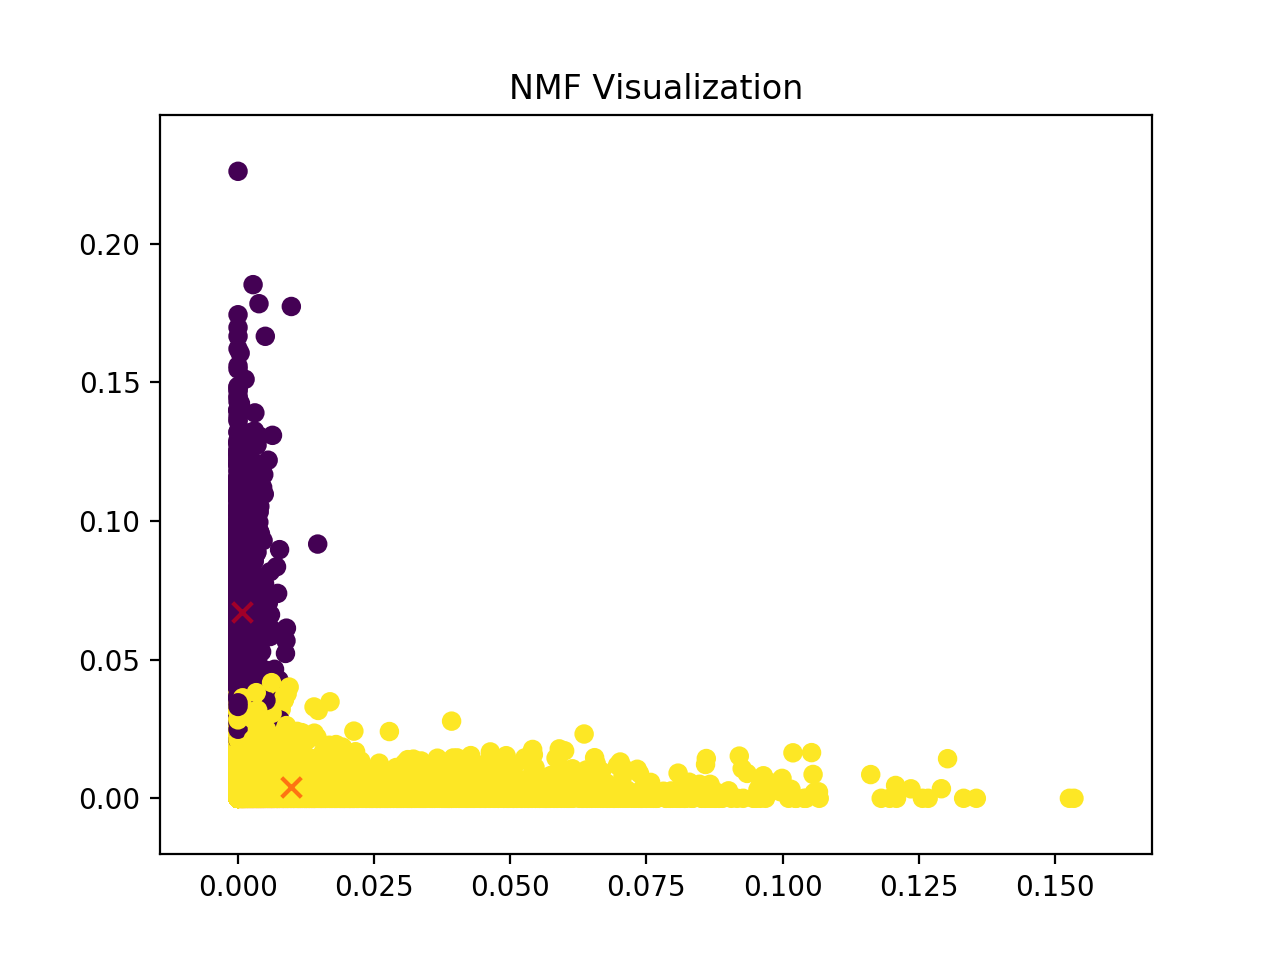
\includegraphics[height=2in]{nmf_clusters_4a.png}}%
\qquad
\subfigure[SVD]{%
\label{fig:svd1}%
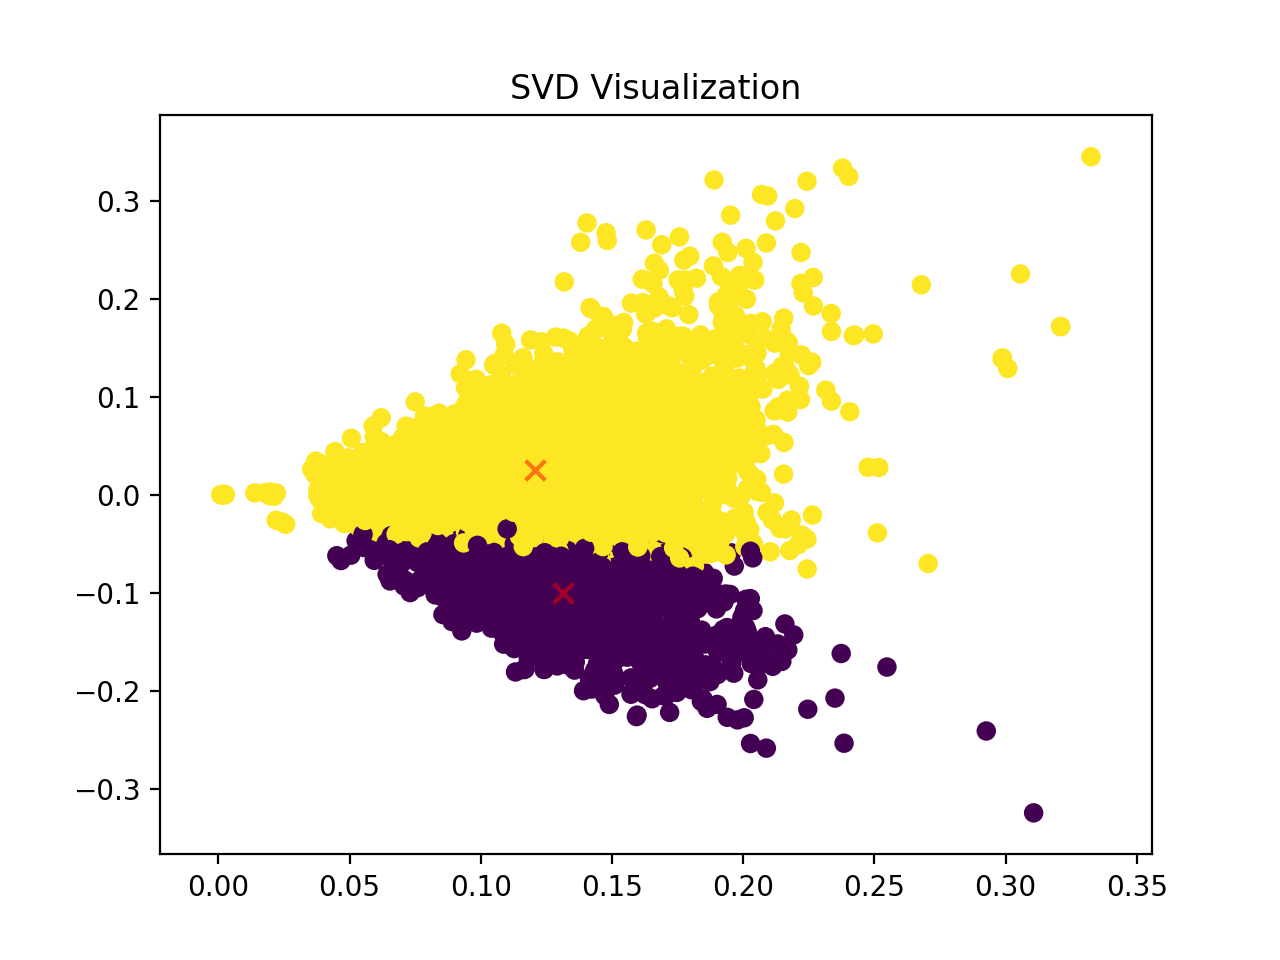
\includegraphics[height=2in]{svd_clusters_4a.png}}%
\vspace*{-3mm}
\caption{Best clustering results for NMF and SVD with color-coded classes}
\end{figure}


%%%%%%%%%%%%%%%%%%%%%%%%%%%%%%%%%%%%%%%%%%%%%%%%%%%%%%%%%%%

\begin{figure}
  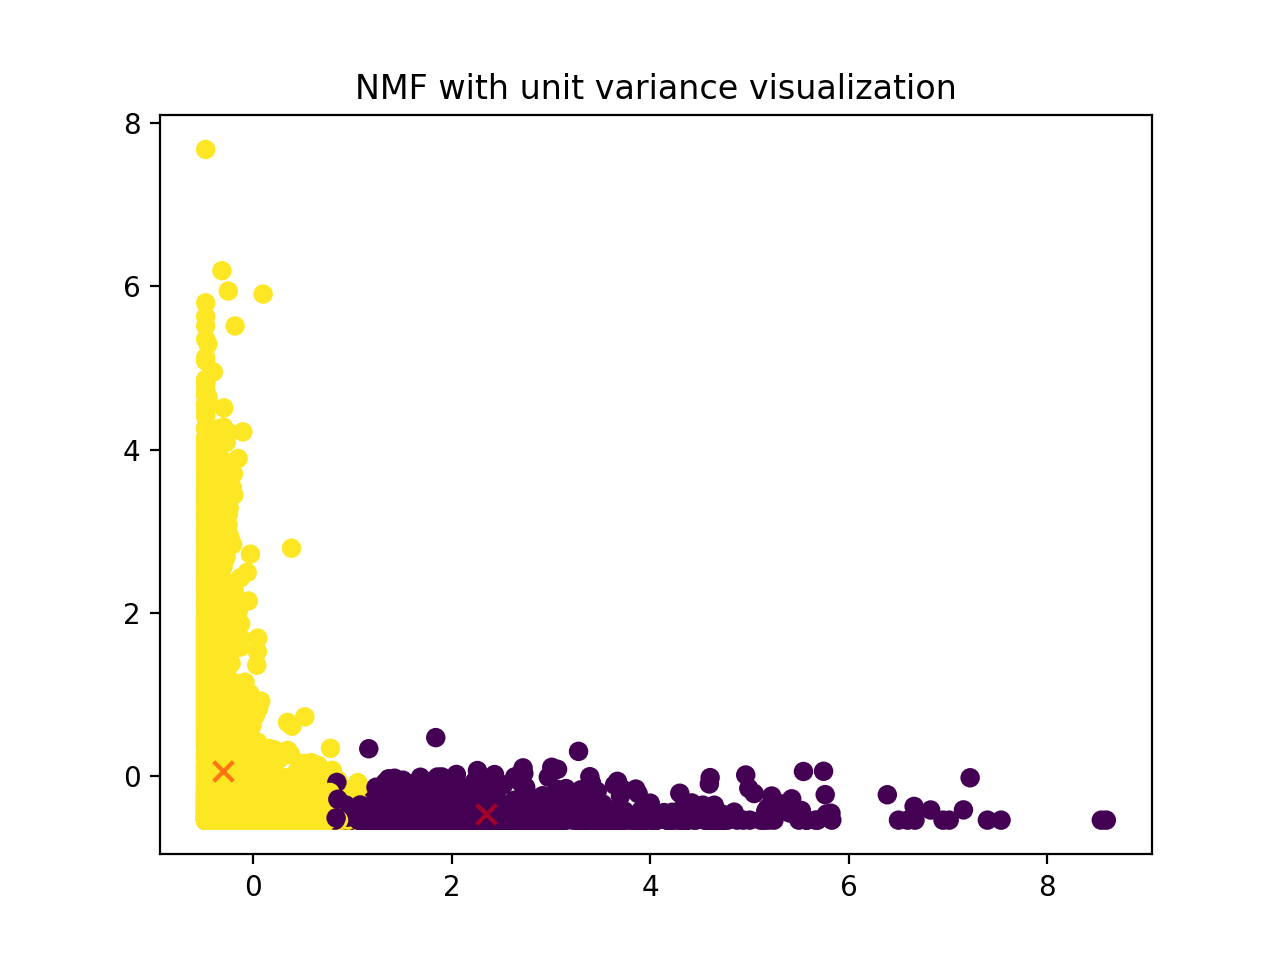
\includegraphics[width=\linewidth]{nmf_unitvar_4b.png} 
  \vspace*{-20mm}
  \caption{Clustering result for NMF with unit variance features}
  \label{fig:nmf2}
\end{figure}

\begin{figure}
  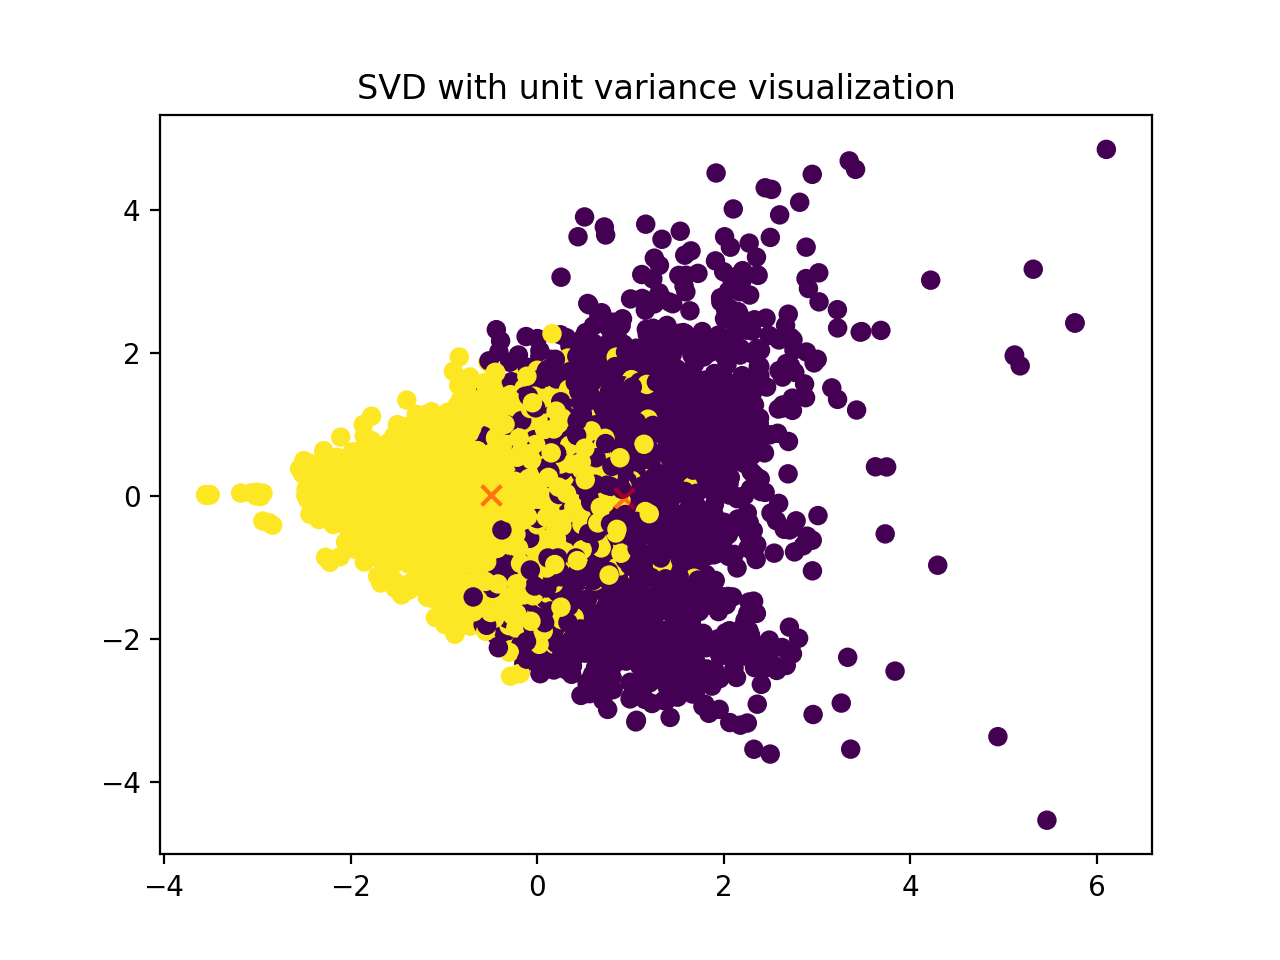
\includegraphics[width=\linewidth]{svd_unitvar_4b.png} 
  \vspace*{-20mm}
  \caption{Clustering result for SVD with unit variance features}
  \label{fig:svd2}
\end{figure}

\begin{figure}
  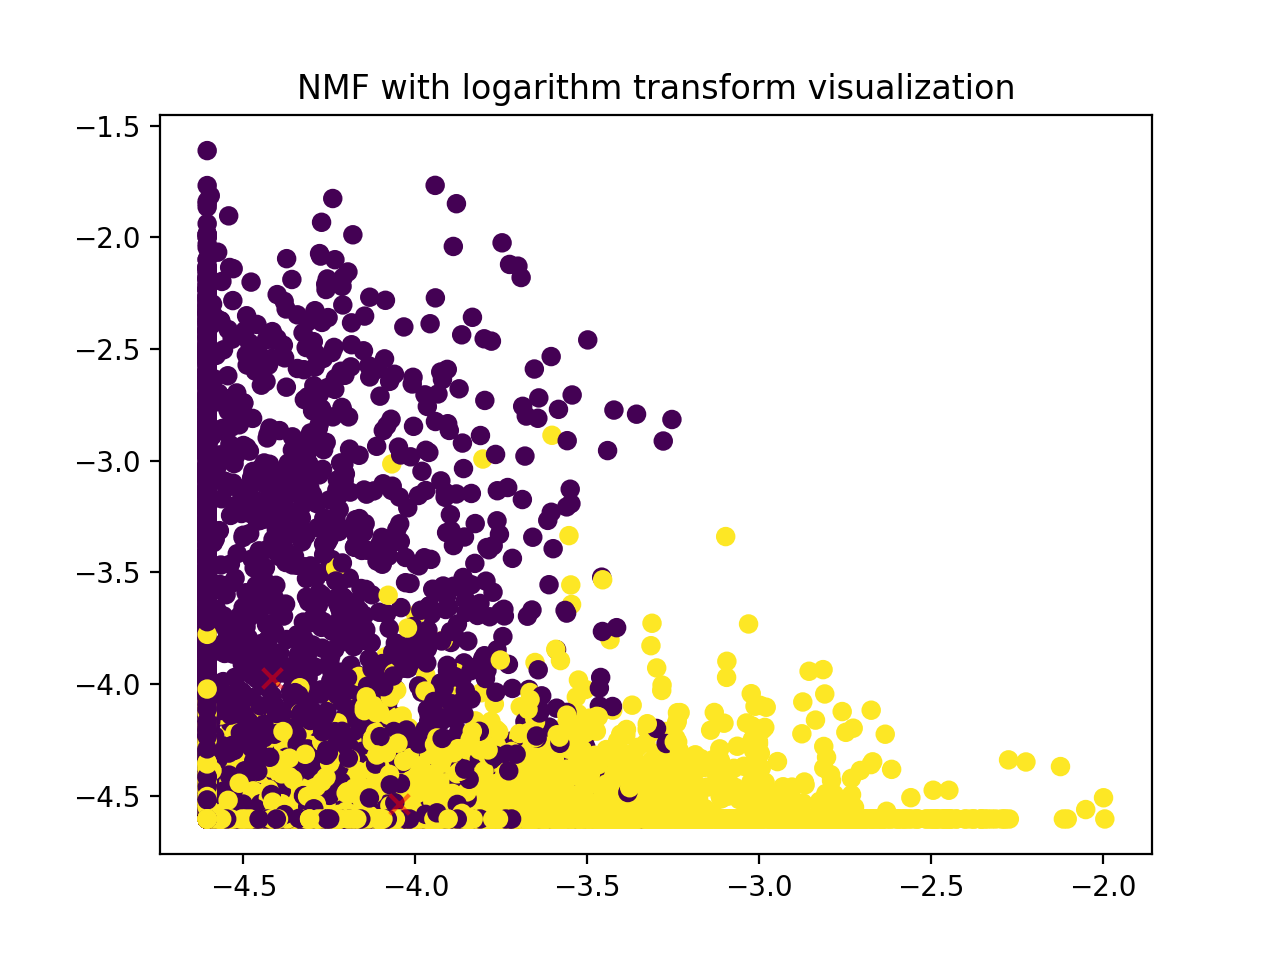
\includegraphics[width=\linewidth]{nmf_log_4b.png} 
  \vspace*{-20mm}
  \caption{Clustering result for NMF with logartihmic transformation}
  \label{fig:nmf3}
\end{figure}

\begin{figure}
  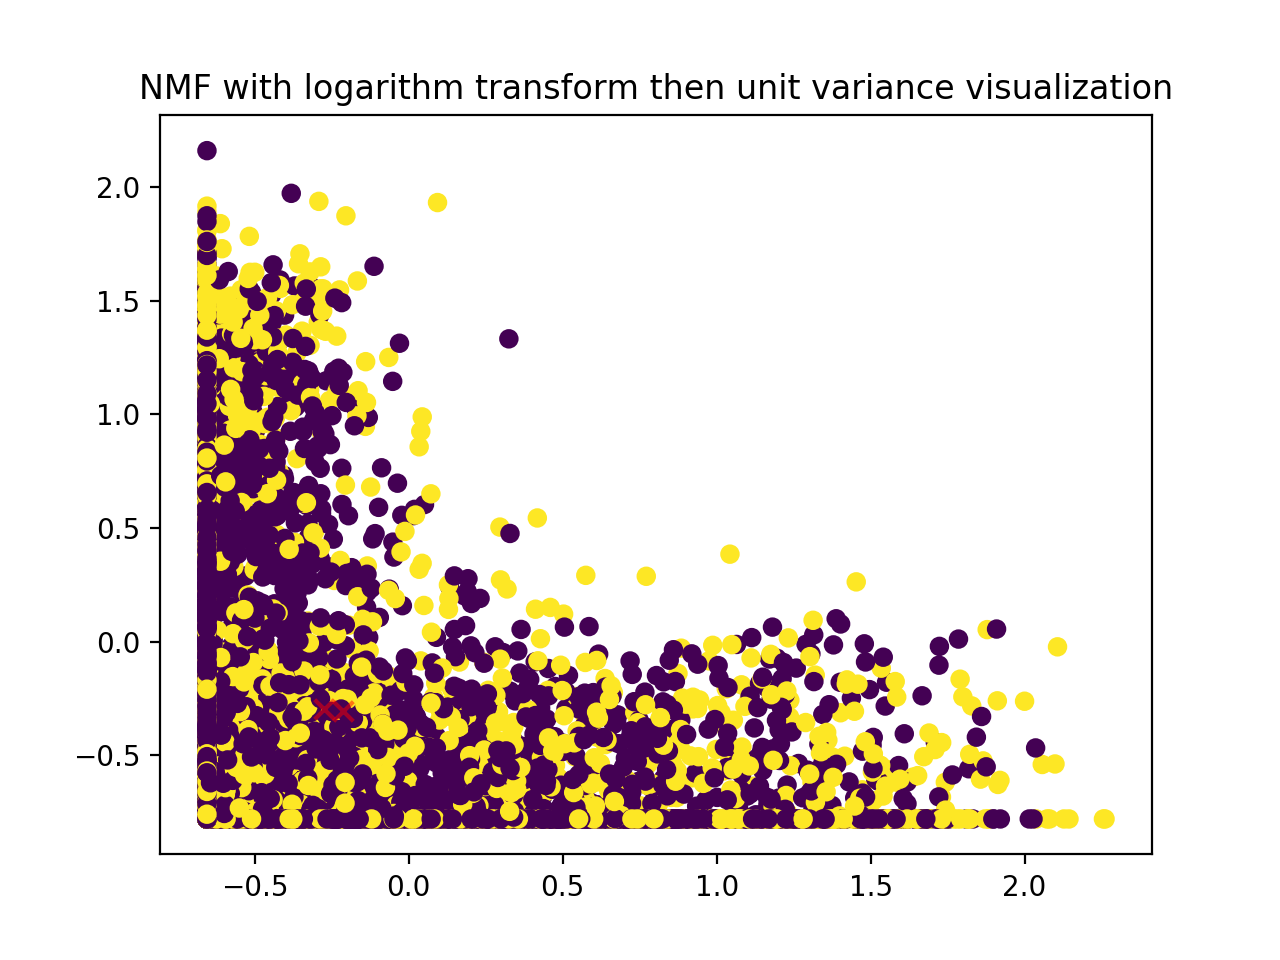
\includegraphics[width=\linewidth]{nmf_log-scalse_4b.png} 
  \vspace*{-20mm}
  \caption{Clustering result for NMF with logarithmic transformation followed by unit variance}
  \label{fig:nmf4}
\end{figure}

\begin{figure}
  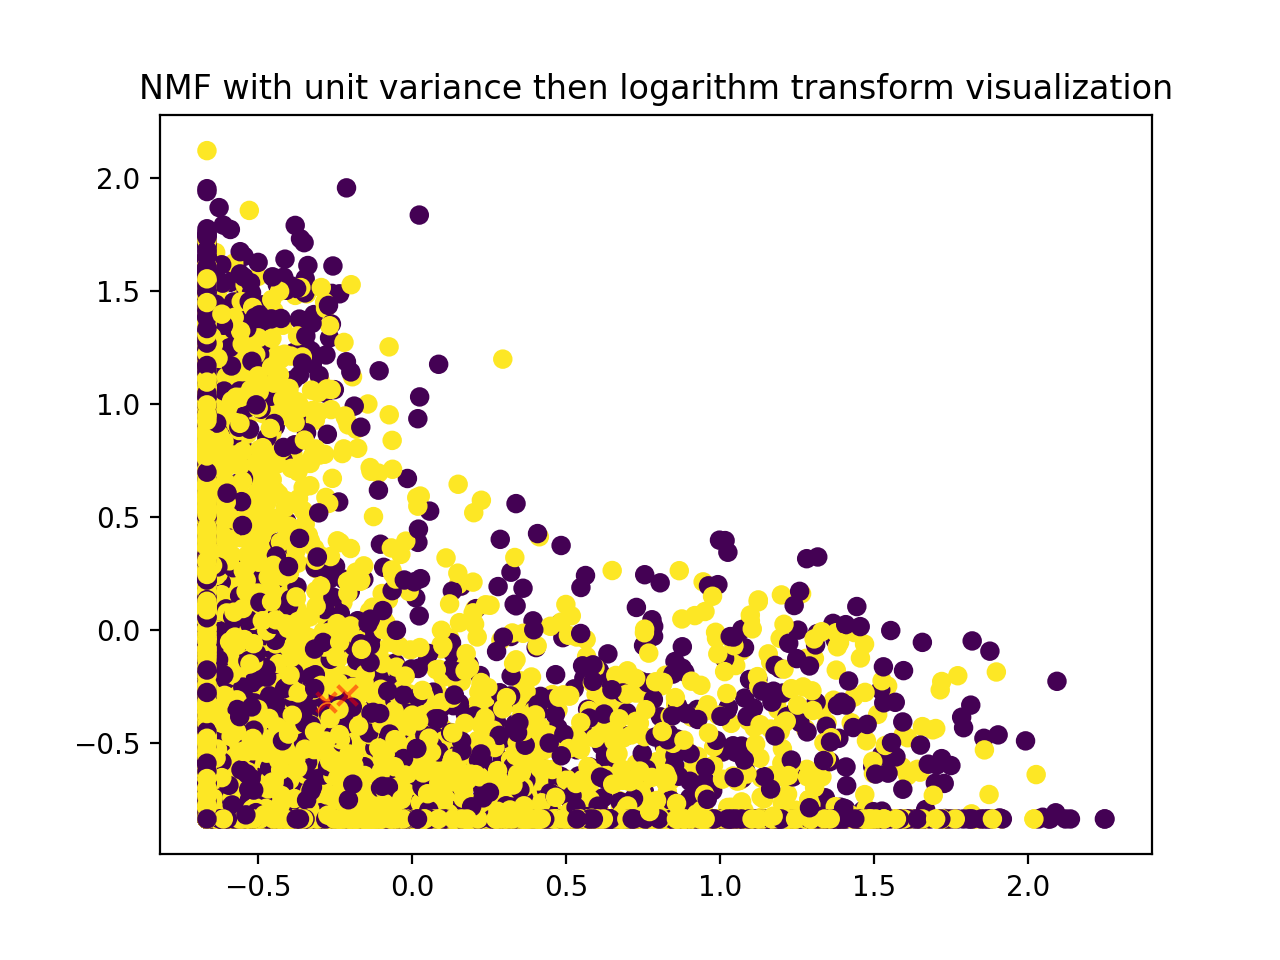
\includegraphics[width=\linewidth]{nmf_scale-log_p4.png} 
  \vspace*{-20mm}
  \caption{Clustering result for NMF with uni variance followed by logarithmic trnasformation}
  \label{fig:nmf5}
\end{figure}


By projecting final data vectors onto 2-dimensional plane and color-coding the classes, the best clustering results from previous part for both SVD and NMF have %been visualized in \ref[fig:svd1} and \ref{fig:nmf1} figures. \\

In effort to improve the performance of the clustering, we used three types of transformation techniques: unit variance of all features, logartihmic trnasformation as a non-linear transformation, and the combination of them. The clustering results after these transformations applied have been illustrated in %\ref{fig: nmf2} through \ref{fig:nmf5}.  Morevoer, the results from all the performance metrics for the clustering with after transformations have been reported below. All these clearly show the improvement in the performance of the clustering. \\ \\



\underline{\textbf{SVD with unit variance}} 

\begin{center}
	\textbf{Performance metrics's scores} \\ \vspace{10pt}	
	\begin{tabular}{*{2}{c}}
		\toprule
		\textbf{Measure} & \textbf{Score} \\		
		\midrule
		Homogeneity: 		& 2.01303068525e-05 \\
		\midrule
		Completeness: 		& 2.14668865991e-05 \\
		\midrule
		V-measure: 			& 2.07771235773e-05 \\
		\midrule
		RAND score: 		& -6.21221803205e-05 \\
		\midrule
		Mutual Info: 		& -7.14202926019e-05 \\
		\bottomrule
	\end{tabular}
	\qquad
	$Contingency = \left[\begin{array}{*{2}{c}}
		1392 		& 2511 \\
		1399 		& 2580 
			\end{array}\right]
		$
\end{center}

\\ \vspace{20pt}

\underline{\textbf{NMF with unit variance}} 

\begin{center}
	\textbf{Performance metrics' scores} \\ \vspace{10pt}		
	\begin{tabular}{*{2}{c}}	
		\toprule
		\textbf{Measure} & \textbf{Score} \\		
		\midrule
		Homogeneity: 		& 0.558580439281 \\
		\midrule
		Completeness: 		& 0.568874068887 \\
		\midrule
		V-measure: 			& 0.563680263802 \\
		\midrule
		RAND score: 		& 0.635981622287 \\
		\midrule
		Mutual Info: 		& 0.558540026933 \\
		\bottomrule
	\end{tabular}
	\qquad	
	$Contingency = \left[ \begin{array}{*{2}{c}}
		692 		& 3211 \\
		3873  		& 106 
			\end{array}\right]
		$
\end{center}
\newpage


\underline{\textbf{NMF with non-linear (log) transform}} 

\begin{center}
	\textbf{Performance metrics' scores} \\ \vspace{10pt}
	\begin{tabular}{*{2}{c}}
		\toprule
		\textbf{Measure} & \textbf{Score} \\
		\midrule
		Homogeneity: 		& 0.730830451039 \\
		\midrule
		Completeness: 		& 0.733210930879 \\
		\midrule
		V-measure: 			& 0.732018755671 \\
		\midrule
		RAND score: 		& 0.815054275835 \\
		\midrule
		Mutual Info: 		& 0.730805808463 \\
		\bottomrule
	\end{tabular}
	\qquad
	$Contingency = \left[\begin{array}{*{2}{c}}
			3597  & 306 \\
			77 	& 3902 
				\end{array}\right]
			$
\end{center}
\\ \vspace{20pt}


\underline{\textbf{NMF with scale then log transform}} 

\begin{center}
	\textbf{Performance metrics' scores} \\ \vspace{10pt}
	\begin{tabular}{*{2}{c}}
		\toprule
		\textbf{Measure} & \textbf{Score} \\
		\midrule
		Homogeneity: & 0.000902761815731 \\
		\midrule
		Completeness: & 0.00090693865041 \\
		\midrule
		V-measure: 	& 0.00090484541295  \\
		\midrule
		RAND score: & 0.00117175851602  \\
		\midrule
		Mutual Info: & 0.000811294034297  \\
		\bottomrule
	\end{tabular}
	\qquad
	$Contingency = \left[\begin{array}{*{2}{c}}
			1864 & 2039\\
			1760 & 2219 
				\end{array}\right]
			$
\end{center}

\newpage

\underline{\textbf{NMF with log transform then scale}}

\begin{center}
	\textbf{Performance metrics' scores for clustering} \\ \vspace{5pt}
	\begin{tabular}{*{2}{c}}			
			\toprule
			\textbf{Measure} & \textbf{Score} \\
			\midrule			
			Homogeneity: & 0.73419145919 \\
			\midrule
			Completeness: & 0.73616241497 \\
			\midrule
			V-measure: & 0.735175616083 \\
			\midrule
			RAND score: & 0.819642953267 \\
			\midrule
			Mutual Info: & 0.734167124321 \\
			\bottomrule
	\end{tabular}
	\qquad
	$Contigency = \left[\begin{array}{*{2}{c}}
		 289 & 3614 \\
	 	 3895 & 84    
		    \end{array}\right]
    $
\end{center}
\\ \vspace{20pt}


\section*{Expansion of Dataset into 20 Categories}
In order to examine how purely we can retrieve all 20 original sub-class labels with clustering, we included all documents and the correspodning terms in the data matrix and figured out proper representation through diemsionality reduction of the TF-IDF representation.

Using the same parameters as in part 1, we tried different dimensions for both truncated SVD and NMF dimensionality reduction. Based on the performance metrics, the best r-values for 20 clusters and 20 sub-classes were found to be as in the following. \\

For 20 clusters, and 20 categories, the best r values have been reported in the table given below. \\


\begin{center}
	\textbf{Best r-values for different performance metrics} \\ \vspace{10pt}
	\begin{tabular}{*{3}{c}}
		\toprule
		\textbf{Performance metric} & \textbf{NMF (r-value)} & \textbf{SVD (r-value)} \\
		\midrule
		Homegeneity & 10 & 10 \\
		\midrule		
		Completeness & 35 & 125 \\
		\midrule		
		V-measure & 35 & 80 \\
		\midrule		
		RAND & 10 & 10   \\
		\midrule
		Mutual info & 10 & 10  \\
		\bottomrule
	\end{tabular}
\end{center}
\\ \vspace{20pt}

After trying with different r-values, we used r=35 for NMF, and r=80 for SVD in order to achieve the best clustering performance. Effects of Scaling and Log transform were observed. Therefore,

\begin{itemize}
	\item SVD
	\begin{itemize}
		\item Scaling worsened results for r=80
	\end{itemize}
    \item NMF
	\begin{itemize}	    
    	\item Scaling worsened results 
		\item Log improved results 
		\item Log then scale improved results the most!
		\item Scale then log worsened results, but not as bad as just scaling	
 	\end{itemize}   
\end{itemize}



\begin{figure}
  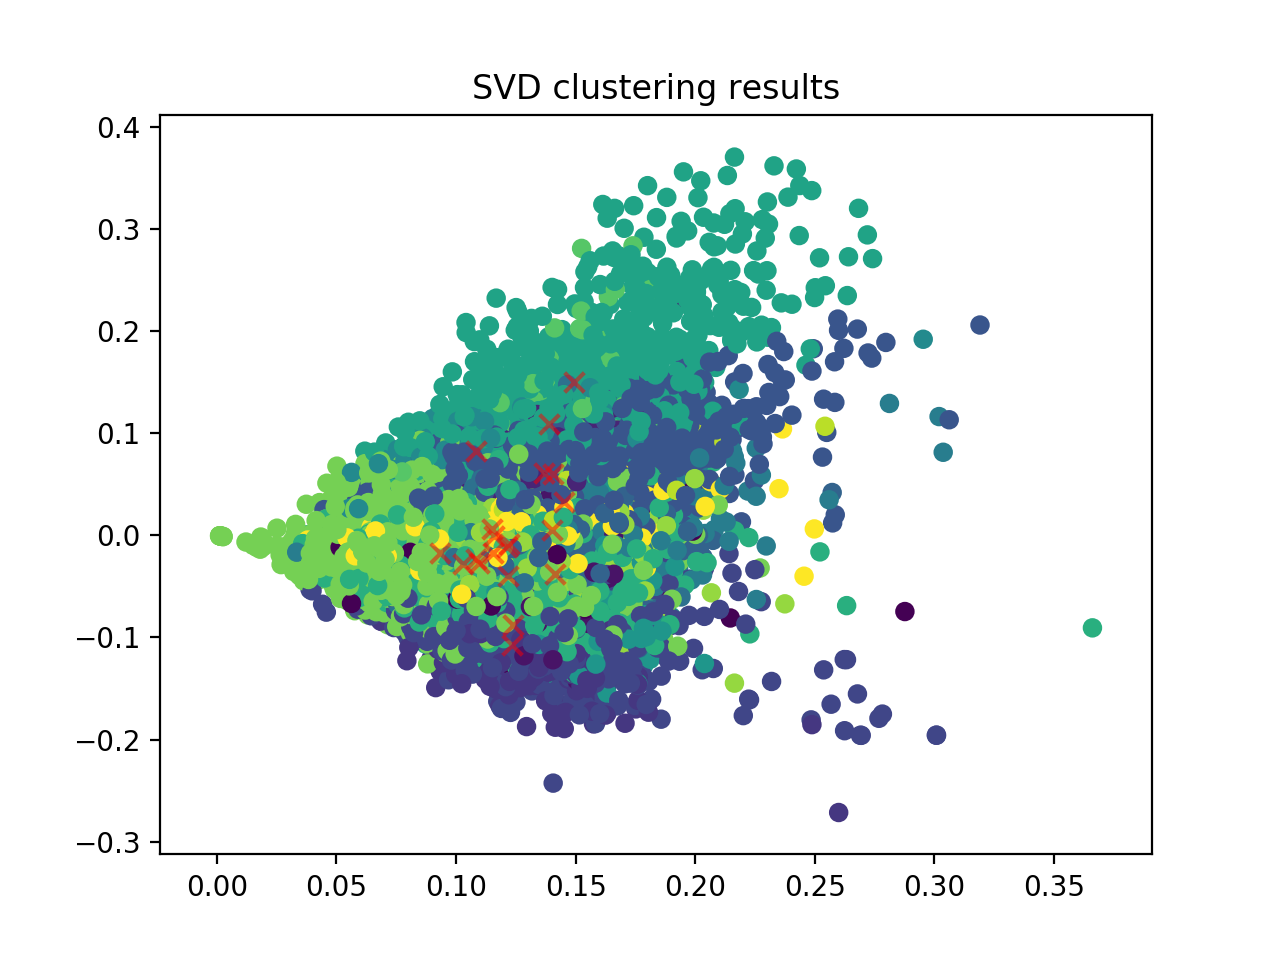
\includegraphics[width=\linewidth]{p5_svd_clustering.png} 
  \vspace*{-20mm}
  \caption{Clustering result for SVD with logarithmic transformation followed by unit variance}
  \label{fig:svd3}
\end{figure}

\\

\begin{figure}
  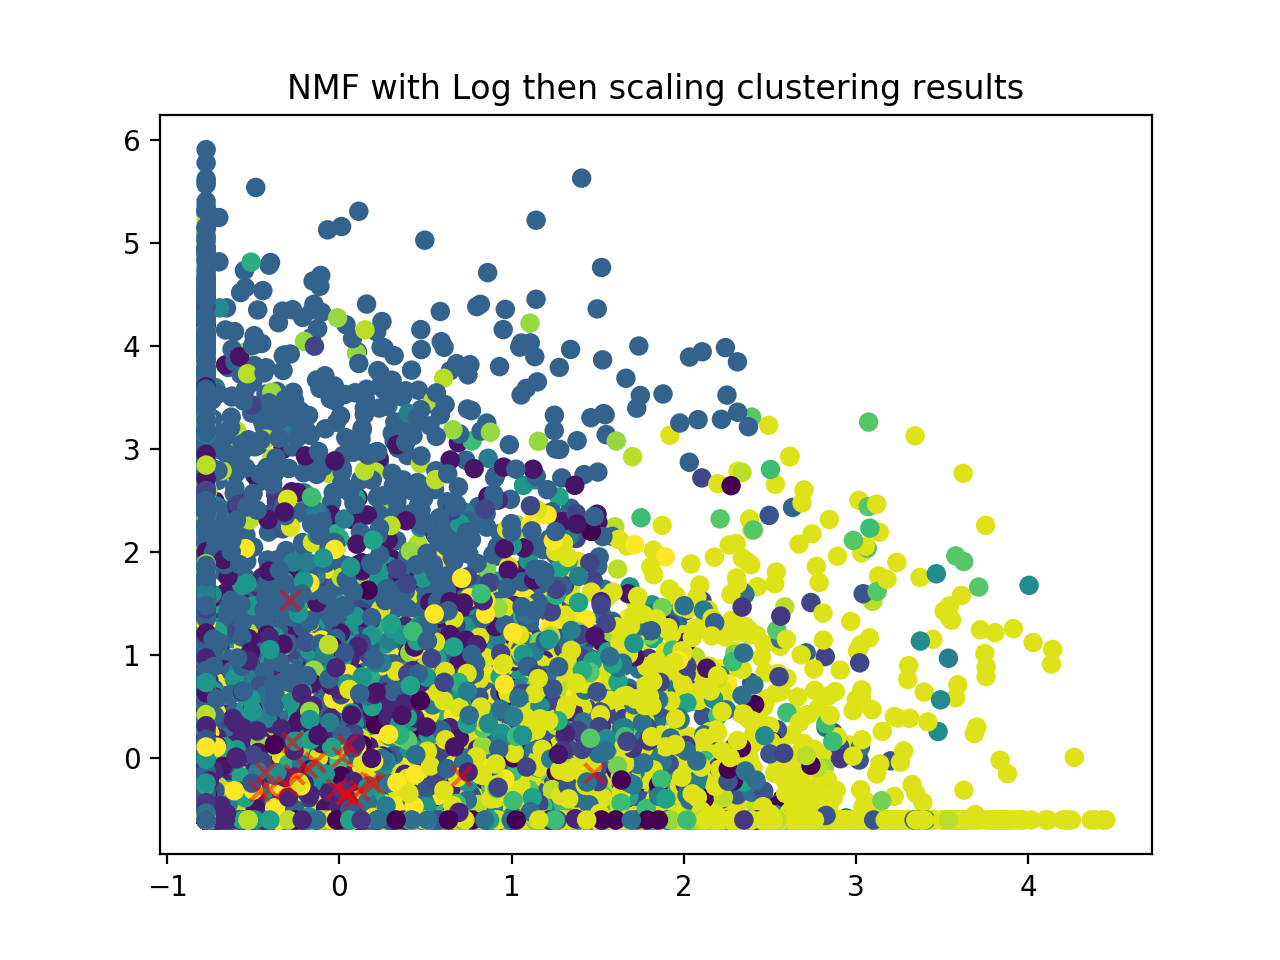
\includegraphics[width=\linewidth]{p5_nmf_clustering.png} 
  \vspace*{-20mm}
  \caption{Clustering result for NMF with logarithmic transformation followed by unit variance}
  \label{fig:nmf6}
\end{figure}


\end{document}
